\documentclass[crop,tikz]{standalone}                 
\usepackage{physics}
\makeatletter                                                                                        

\begin{document}

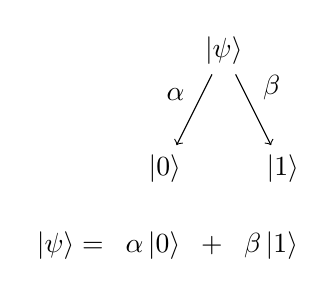
\begin{tikzpicture}[scale=1.5]                                                                          
%\draw [dotted] (-1,-1) grid (1, 1);
\node []   (nodeX) at ( 0.50,  1.00) {$\ket{\psi}$}     ;                                          
\node []   (node0) at ( 0.00,  0.00) {$\ket{0}$}        ;                                          
\node []   (node1) at ( 1.00,  0.00) {$\ket{1}$}        ;                                       
\node []   (nodea) at (-0.80, -0.65) {$\ket{\psi}=$}    ;                                          
\node []   (nodea) at (-0.10, -0.65) {$\alpha \ket{0}$} ;                                          
\node []   (nodep) at ( 0.40, -0.65) {$+$}              ;                                          
\node []   (nodeb) at ( 0.90, -0.65) {$\beta  \ket{1}$} ;                                       
\draw [->] (nodeX) -- (node0) node[midway, above left  ] {$\alpha$} ;                                                           
\draw [->] (nodeX) -- (node1) node[midway, above right ] {$\beta$}  ; 
\end{tikzpicture}                                                                                    

\end{document}
